\documentclass[journal]{IEEEtran}

\usepackage[utf8]{inputenc}
\usepackage{amsmath,amssymb,amsfonts}
\usepackage{graphicx}
\usepackage{textcomp}
\usepackage{xcolor}
\usepackage{booktabs}
\usepackage{multirow}
\usepackage{hyperref}
\usepackage{cite}
\usepackage{caption}

\graphicspath{{../results/plots/}}

\begin{document}

\title{Federated Learning Under Data and System Heterogeneity: An Experimental Evaluation of FedAvg Across Non-IID Settings}

\author{
% TODO: Add your group members here
Member~1,~Member~2,~Member~3,~Member~4
\thanks{Category 7: System Heterogeneity. Course: Federated Learning, BDS Program, IIT Patna, Jan--April 2026.}
}

\maketitle

\begin{abstract}
Federated learning (FL) enables collaborative model training across distributed devices without centralizing raw data. However, heterogeneity in data distributions, client populations, and device capabilities poses significant challenges to convergence and model quality. In this paper, we conduct a systematic experimental evaluation of the Federated Averaging (FedAvg) algorithm under varying degrees of data heterogeneity and client scale, guided by the heterogeneity taxonomy of Chen et al.~\cite{chen2025advances}. Using the Flower simulation framework, we evaluate FedAvg on MNIST, Fashion-MNIST, and CIFAR-10 with Dirichlet-based non-IID partitioning ($\alpha \in \{0.01, 0.1, 0.5, 1.0, \text{IID}\}$) and client scales of 10, 50, and 100. Our experiments quantify the accuracy degradation caused by data heterogeneity, reveal how increasing client counts amplifies the non-IID effect under partial participation, and identify the heterogeneity regimes where FedAvg remains effective versus where more advanced methods are needed.
\end{abstract}

\begin{IEEEkeywords}
Federated learning, data heterogeneity, non-IID data, FedAvg, Dirichlet partitioning
\end{IEEEkeywords}

%% ============================================================
\section{Introduction}
\label{sec:intro}

The proliferation of mobile devices and Internet of Things (IoT) sensors has led to an unprecedented volume of data generated at the network edge. Traditional centralized machine learning requires aggregating this data on a central server, raising serious concerns about data privacy, communication overhead, and regulatory compliance. Federated learning (FL), first proposed by McMahan et al.~\cite{mcmahan2017communication}, addresses these challenges by enabling multiple clients to collaboratively train a shared model while keeping data localized on each device.

In the canonical FL protocol, Federated Averaging (FedAvg), a central server coordinates training over multiple communication rounds. In each round, a subset of clients downloads the current global model, performs local training on their private data, and uploads updated model parameters to the server, which aggregates them via weighted averaging. While elegant in principle, FedAvg assumes relatively homogeneous conditions---an assumption that rarely holds in practice.

Chen et al.~\cite{chen2025advances} present a comprehensive taxonomy of heterogeneity in federated learning, identifying five key dimensions: data heterogeneity, model heterogeneity, task heterogeneity, communication heterogeneity, and device heterogeneity. Of these, \textbf{data heterogeneity}---where clients have non-identically distributed (non-IID) local datasets---is perhaps the most fundamental challenge, as it directly affects the quality of locally trained models and the effectiveness of aggregation.

In this paper, we focus on understanding the empirical impact of data heterogeneity on FedAvg across multiple axes: the degree of label skew (controlled by the Dirichlet concentration parameter $\alpha$), the number of participating clients, and the dataset complexity. Rather than proposing a new algorithm, we aim to systematically characterize \textit{when and how much} heterogeneity degrades FedAvg performance, providing a baseline understanding that motivates the need for more advanced methods surveyed in~\cite{chen2025advances}.

Our contributions are: (1) we review the heterogeneity taxonomy of Chen et al.~\cite{chen2025advances} and contextualize it within the FL literature; (2) we conduct a systematic experimental evaluation of FedAvg across 22 configurations spanning 3 datasets, 3 client scales, and 5 heterogeneity levels; (3) we analyze how data heterogeneity interacts with client scale and dataset complexity; and (4) we identify the heterogeneity thresholds beyond which FedAvg fails to converge, motivating the need for techniques such as proximal regularization, client selection, and asynchronous aggregation.


%% ============================================================
\section{Literature Review}
\label{sec:litreview}

\subsection{Advances in Robust Federated Learning (Chen et al., 2025)}

Chen et al.~\cite{chen2025advances} present a comprehensive survey of heterogeneous federated learning, systematically categorizing challenges and solutions across five dimensions.

\subsubsection{Taxonomy of Heterogeneity}

\textbf{Data heterogeneity} encompasses distribution skew (non-IID data where $P_i(x,y) \neq P_j(x,y)$), label skew (differing label distributions across clients), feature skew (different feature representations), quality skew (varying data quality), and quantity skew (imbalanced dataset sizes). The Dirichlet distribution with parameter $\alpha$ is commonly used to model label distribution skew, where smaller $\alpha$ values produce more heterogeneous partitions~\cite{hsu2019measuring}.

\textbf{Model heterogeneity} includes structural heterogeneity, where clients employ different model architectures due to varying hardware capabilities, and optimizer heterogeneity, where clients use different optimization algorithms or hyperparameters.

\textbf{Task heterogeneity} arises when clients face different learning tasks or objective functions, requiring the system to balance global generalizability and client-specific personalization.

\textbf{Communication heterogeneity} reflects differences in network bandwidth, latency, and connection stability across clients.

\textbf{Device heterogeneity} captures variability in computing power, storage, and energy resources, directly affecting local training speed and the straggler problem.

\subsubsection{Methods Addressing Heterogeneity}

The survey organizes solutions into three levels:

\textit{Data-level methods} include data augmentation techniques like FRAug and StatMix to enhance local data diversity, and representation learning approaches such as MOON and FedProto.

\textit{Model-level methods} modify model parameters or architectures. FedProx~\cite{li2020federated} adds a proximal term to prevent client drift. SCAFFOLD~\cite{karimireddy2020scaffold} uses control variates to correct for heterogeneity-induced drift. Model compression through sparsification and quantization reduces communication overhead.

\textit{Architecture-level methods} adjust the training structure itself. Client selection mechanisms (FedCS~\cite{nishio2019client}, Oort~\cite{lai2021oort}) intelligently choose participants. Asynchronous FL methods like FedBuff~\cite{nguyen2022federated} decouple client updates from global synchronization. Clustered FL groups clients with similar data distributions.

\subsubsection{Privacy in Heterogeneous FL}

The survey notes that heterogeneous settings can exacerbate privacy vulnerabilities. Differential privacy mechanisms add calibrated noise but face challenges when clients have varying privacy requirements. Secure multi-party computation provides stronger guarantees but incurs high computational overhead.


%% ============================================================
\section{Related Work}
\label{sec:related}

\subsection{FedAvg and Its Limitations}

FedAvg~\cite{mcmahan2017communication} remains the most widely used FL algorithm due to its simplicity. However, its convergence guarantees rely on the assumption that local data distributions are approximately IID. Li et al.~\cite{li2020federated} demonstrated that FedAvg diverges under extreme non-IID conditions and proposed FedProx to address this via proximal regularization. SCAFFOLD~\cite{karimireddy2020scaffold} provides stronger convergence guarantees by correcting for client drift using control variates.

\subsection{Measuring and Modeling Non-IID Data}

Hsu et al.~\cite{hsu2019measuring} introduced the use of Dirichlet-based partitioning to systematically control the degree of non-IID in FL experiments. The concentration parameter $\alpha$ controls heterogeneity: $\alpha \to 0$ produces extreme label skew (each client has data from only one or two classes), while $\alpha \to \infty$ approximates IID. This approach has become the standard for benchmarking FL algorithms under data heterogeneity.

\subsection{System Heterogeneity and Stragglers}

System heterogeneity---variability in client computation speed, memory, and network---manifests through the straggler problem in synchronous FL~\cite{bonawitz2019towards}. Asynchronous methods~\cite{xu2023asynchronous,nguyen2022federated,wu2020safa} allow the server to aggregate updates without waiting for all clients. Wang et al.~\cite{wang2025decentralized} propose FedDgc with a dynamically growing cache for asynchronous FL on edge devices. Client selection~\cite{nishio2019client,lai2021oort} and partial training~\cite{zhang2023timelyfl} offer alternative approaches.


%% ============================================================
\section{Methodology}
\label{sec:methodology}

\subsection{FedAvg Protocol}

Our implementation follows the standard FedAvg protocol from McMahan et al.~\cite{mcmahan2017communication}. In each round $t$, the server samples a fraction $C = 0.5$ of available clients, distributes the current global model $w^t$, and aggregates returned updates via weighted averaging:
\begin{equation}
    w^{t+1} = \sum_{k=1}^{K} \frac{n_k}{n} w_k^t
\end{equation}
where $n_k$ is the number of training samples on client $k$ and $n = \sum_k n_k$.

\subsection{Non-IID Data Partitioning}

We use the Dirichlet distribution to partition data across clients. For each class $c$, we draw a probability vector $\mathbf{p}_c \sim \text{Dir}(\alpha)$ and assign data points of class $c$ to clients according to $\mathbf{p}_c$. The concentration parameter $\alpha$ controls heterogeneity:

\begin{itemize}
    \item $\alpha = 0.01$: Extreme non-IID. Most clients have data from only 1--2 classes.
    \item $\alpha = 0.1$: High non-IID. Clients have skewed label distributions with 2--4 dominant classes.
    \item $\alpha = 0.5$: Moderate non-IID. Clients have data from most classes but with varying proportions.
    \item $\alpha = 1.0$: Mild non-IID. Label distributions are mildly skewed.
    \item IID: Uniform random partitioning with balanced label distributions.
\end{itemize}

The Flower Datasets library handles partitioning via \texttt{DirichletPartitioner}. Each client's local data is split 80/20 for training and evaluation.

\subsection{CNN Model Architecture}

We use a lightweight CNN with four convolutional layers (32, 64, 128, 128 filters with $3 \times 3$ kernels), two max-pooling layers, and two fully connected layers (256 units, then $C$ output classes). Dropout ($p=0.25$) is applied before the output layer. The model is adapted for each dataset's input dimensions (grayscale $28 \times 28$ for MNIST/FMNIST, RGB $32 \times 32$ for CIFAR-10).


%% ============================================================
\section{Experimental Setup}
\label{sec:setup}

\subsection{Datasets}

We evaluate on three standard image classification benchmarks:
\begin{itemize}
    \item \textbf{MNIST}~\cite{lecun1998gradient}: 60,000/10,000 grayscale images ($28 \times 28$) of handwritten digits (10 classes).
    \item \textbf{Fashion-MNIST}~\cite{xiao2017fashion}: 60,000/10,000 grayscale images ($28 \times 28$) of clothing items (10 classes).
    \item \textbf{CIFAR-10}~\cite{krizhevsky2009learning}: 50,000/10,000 color images ($32 \times 32$) across 10 object categories.
\end{itemize}

These datasets span increasing complexity: MNIST (simple, well-separated classes), Fashion-MNIST (moderate, visually similar classes), and CIFAR-10 (complex, natural images).

\subsection{Experimental Configurations}

We run 22 experiments across:
\begin{itemize}
    \item \textbf{Datasets:} CIFAR-10 (11 configs), Fashion-MNIST (9 configs), MNIST (2 configs).
    \item \textbf{Client scales:} 10, 50, 100.
    \item \textbf{Heterogeneity:} $\alpha \in \{0.01, 0.1, 0.5, 1.0, \text{IID}\}$.
\end{itemize}

\subsection{Hyperparameters}

Table~\ref{tab:hyperparams} summarizes the experimental configuration.

\begin{table}[h]
\centering
\caption{Experimental hyperparameters.}
\label{tab:hyperparams}
\begin{tabular}{ll}
\toprule
\textbf{Parameter} & \textbf{Value} \\
\midrule
Number of clients & 10, 50, 100 \\
Client fraction per round ($C$) & 0.5 \\
Communication rounds & 100 \\
Local epochs & 5 \\
Batch size & 32 \\
Optimizer & SGD (momentum = 0.9) \\
Learning rate & 0.01 \\
Random seed & 42 \\
\bottomrule
\end{tabular}
\end{table}

\subsection{Evaluation Metrics}

We report: (1) \textit{Global test accuracy} evaluated every round on a held-out test set; (2) \textit{Global test loss} (cross-entropy); (3) \textit{Convergence round}---the first round at which accuracy exceeds 80\%; (4) \textit{Communication cost} computed as model size $\times$ participating clients per round $\times$ rounds $\times$ 2.


%% ============================================================
\section{Results and Analysis}
\label{sec:results}

\subsection{Summary of Results}

Table~\ref{tab:results} presents the summary of experimental results across all configurations.

\begin{table*}[t]
\centering
\caption{Summary of FedAvg experimental results. Convergence round = first round to reach 80\% accuracy ($-1$ if not reached within 100 rounds).}
\label{tab:results}
\begin{tabular}{lcccc}
\toprule
\textbf{Dataset / Clients / $\alpha$} & \textbf{Test Acc. (\%)} & \textbf{Final Loss} & \textbf{Conv. Round} & \textbf{Acc. Drop vs. IID (\%)} \\
\midrule
\multicolumn{5}{l}{\textit{CIFAR-10, 10 clients}} \\
\quad IID     & 70.02 & 0.943 & --  & --- \\
\quad $\alpha=0.5$  & 63.90 & 1.088 & --  & 6.12 \\
\quad $\alpha=0.1$  & 57.13 & 1.297 & --  & 12.89 \\
\midrule
\multicolumn{5}{l}{\textit{CIFAR-10, 50 clients}} \\
\quad IID     & 66.14 & 1.019 & --  & --- \\
\quad $\alpha=0.5$  & 62.17 & 1.152 & --  & 3.97 \\
\quad $\alpha=0.1$  & 53.13 & 1.449 & --  & 13.01 \\
\midrule
\multicolumn{5}{l}{\textit{CIFAR-10, 100 clients}} \\
\quad IID     & 63.87 & 1.082 & --  & --- \\
\quad $\alpha=1.0$  & 62.35 & 1.133 & --  & 1.52 \\
\quad $\alpha=0.5$  & 59.11 & 1.245 & --  & 4.76 \\
\quad $\alpha=0.1$  & 49.32 & 1.538 & --  & 14.55 \\
\quad $\alpha=0.01$ & 38.13 & 1.844 & --  & 25.74 \\
\midrule
\multicolumn{5}{l}{\textit{Fashion-MNIST, 10 clients}} \\
\quad IID     & 89.06 & 0.325 & 35  & --- \\
\quad $\alpha=0.5$  & 86.06 & 0.390 & 42  & 3.00 \\
\quad $\alpha=0.1$  & 82.47 & 0.506 & 53  & 6.59 \\
\midrule
\multicolumn{5}{l}{\textit{Fashion-MNIST, 50 clients}} \\
\quad IID     & 88.20 & 0.321 & 34  & --- \\
\quad $\alpha=0.5$  & 84.79 & 0.418 & 40  & 3.41 \\
\quad $\alpha=0.1$  & 79.30 & 0.592 & 87  & 8.90 \\
\midrule
\multicolumn{5}{l}{\textit{Fashion-MNIST, 100 clients}} \\
\quad IID     & 86.95 & 0.394 & 33  & --- \\
\quad $\alpha=0.5$  & 83.28 & 0.473 & 41  & 3.67 \\
\quad $\alpha=0.1$  & 77.95 & 0.658 & --  & 9.00 \\
\midrule
\multicolumn{5}{l}{\textit{MNIST, 100 clients}} \\
\quad IID     & 99.49 & 0.046 & 16  & --- \\
\quad $\alpha=0.1$  & 96.32 & 0.131 & 24  & 3.17 \\
\bottomrule
\end{tabular}
\end{table*}

\subsection{Effect of Data Heterogeneity}

Figure~\ref{fig:accuracy_alpha} shows the global test accuracy vs.\ communication rounds for CIFAR-10 with 100 clients under varying $\alpha$.

\begin{figure}[h]
\centering
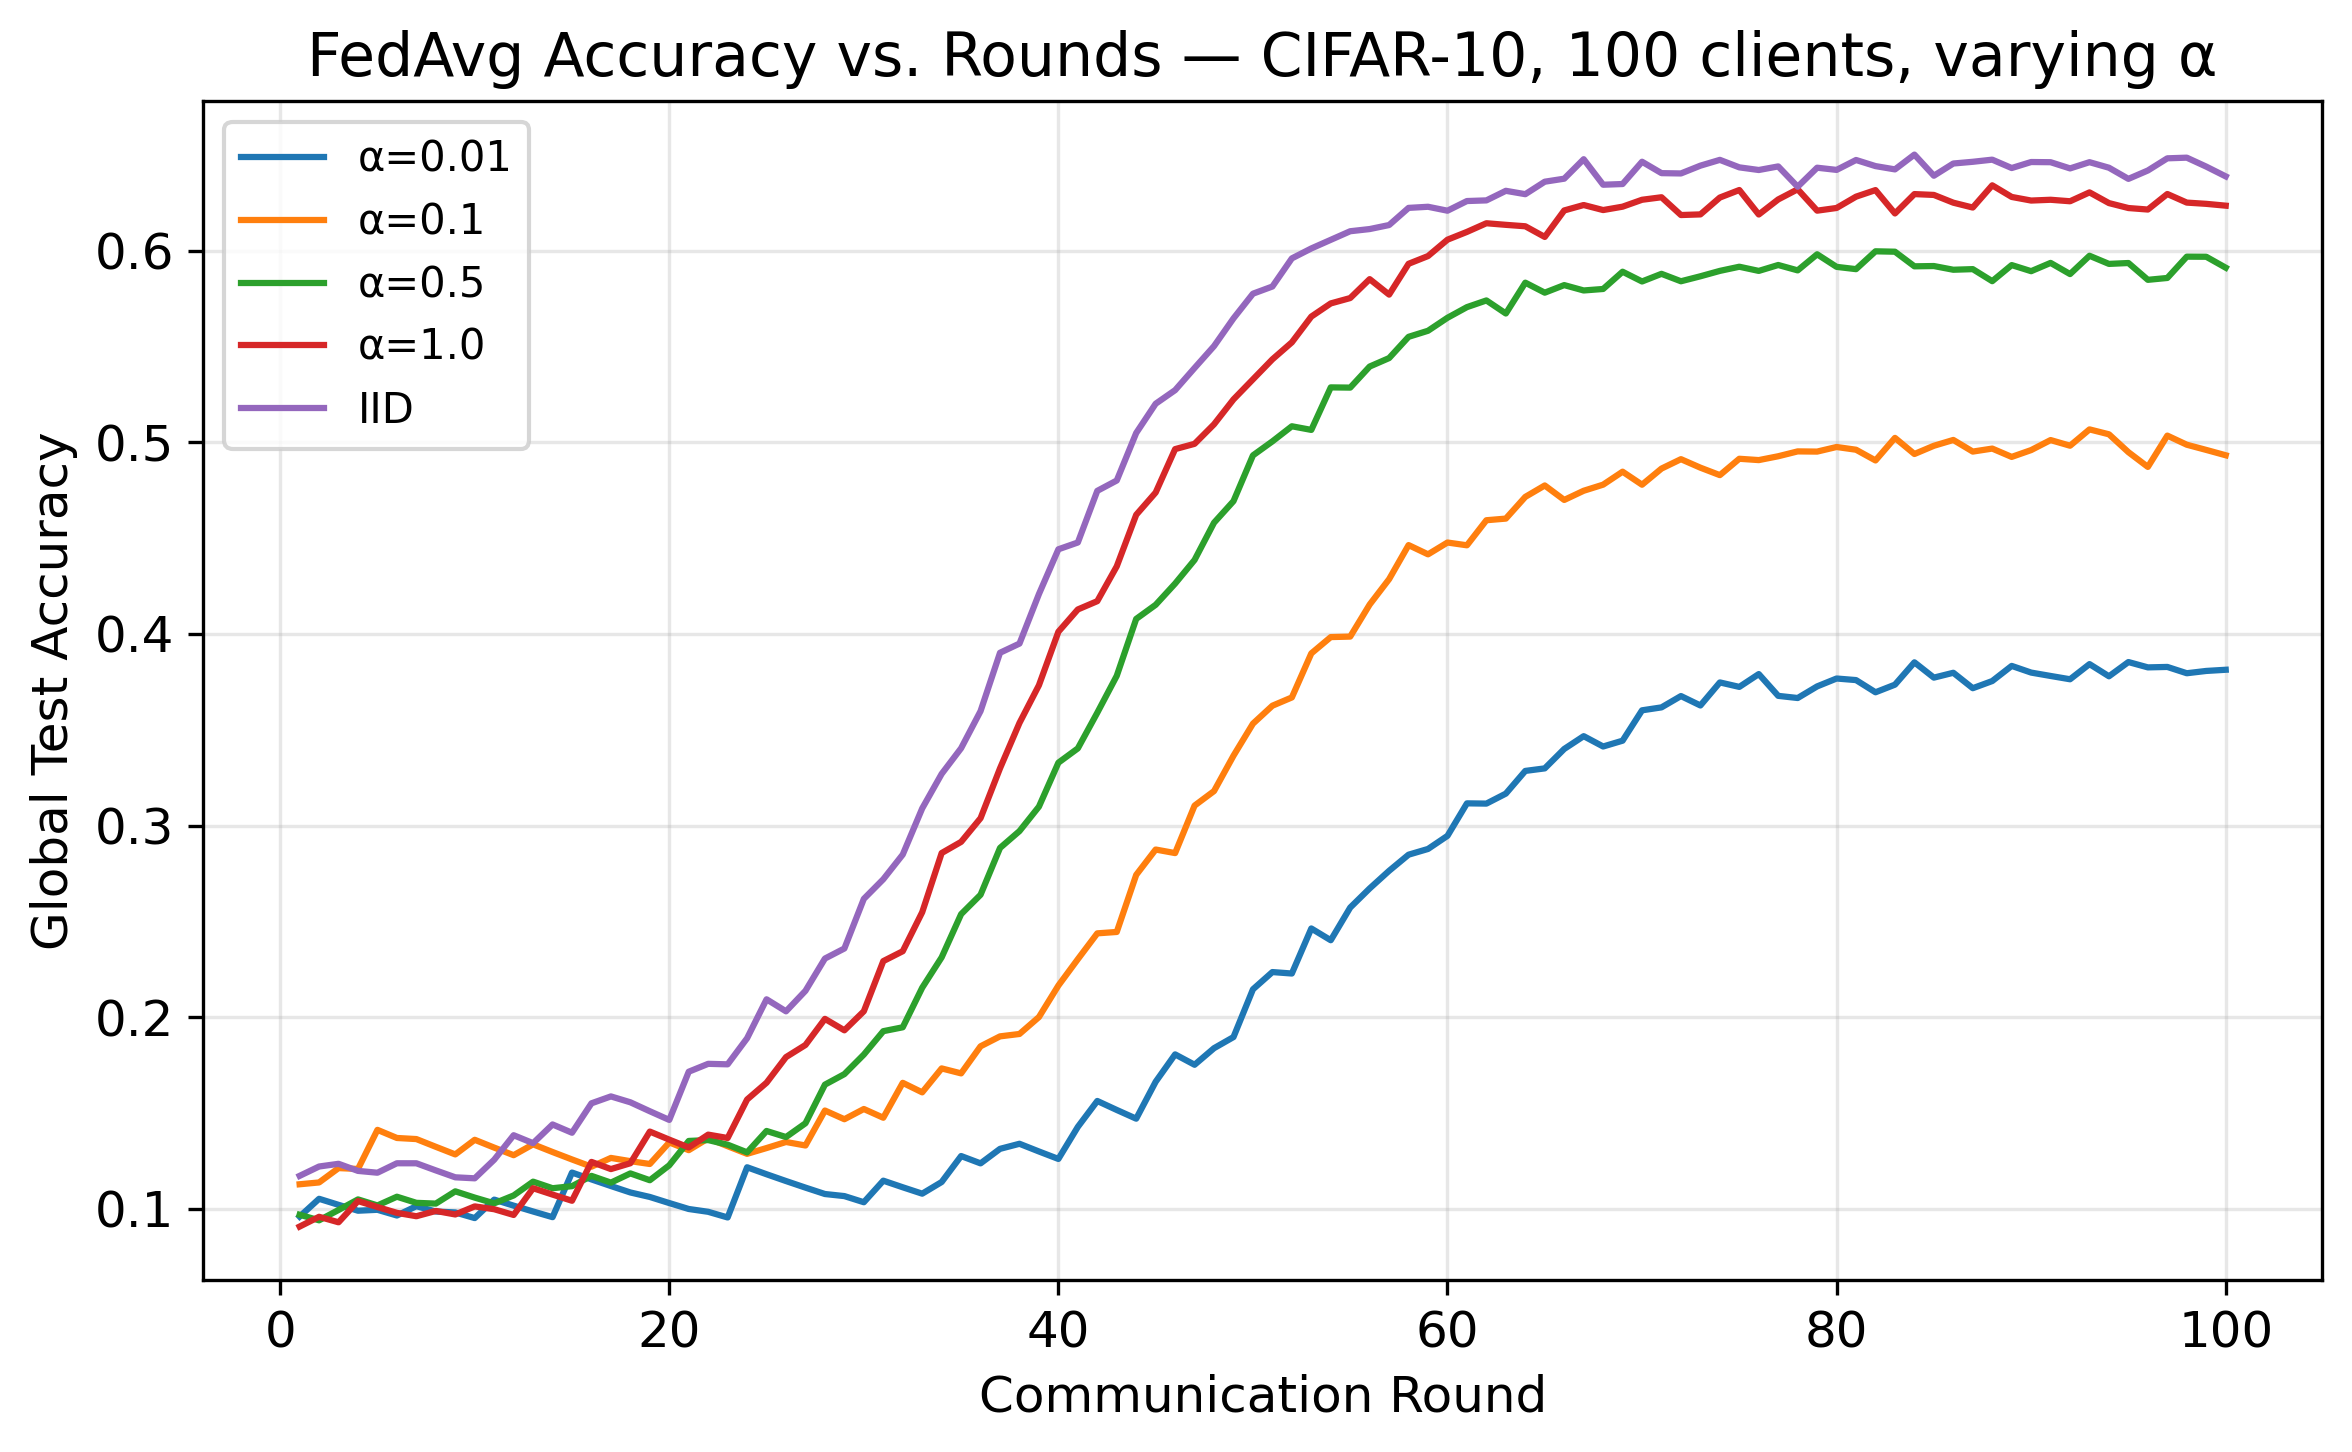
\includegraphics[width=\columnwidth]{accuracy_vs_alpha_cifar10_c100.png}
\caption{FedAvg accuracy vs.\ communication rounds on CIFAR-10 (100 clients) under varying Dirichlet $\alpha$. Lower $\alpha$ values (more heterogeneous) lead to significantly lower final accuracy and slower convergence.}
\label{fig:accuracy_alpha}
\end{figure}

The results clearly demonstrate that data heterogeneity has a substantial impact on FedAvg performance. On CIFAR-10 with 100 clients, moving from IID to $\alpha=0.1$ causes a 14.55\% accuracy drop, and extreme heterogeneity ($\alpha=0.01$) results in a 25.74\% drop. The loss curves (Figure~\ref{fig:loss_alpha}) corroborate this trend, with more heterogeneous settings exhibiting higher final loss values and more oscillatory convergence behavior.

\begin{figure}[h]
\centering
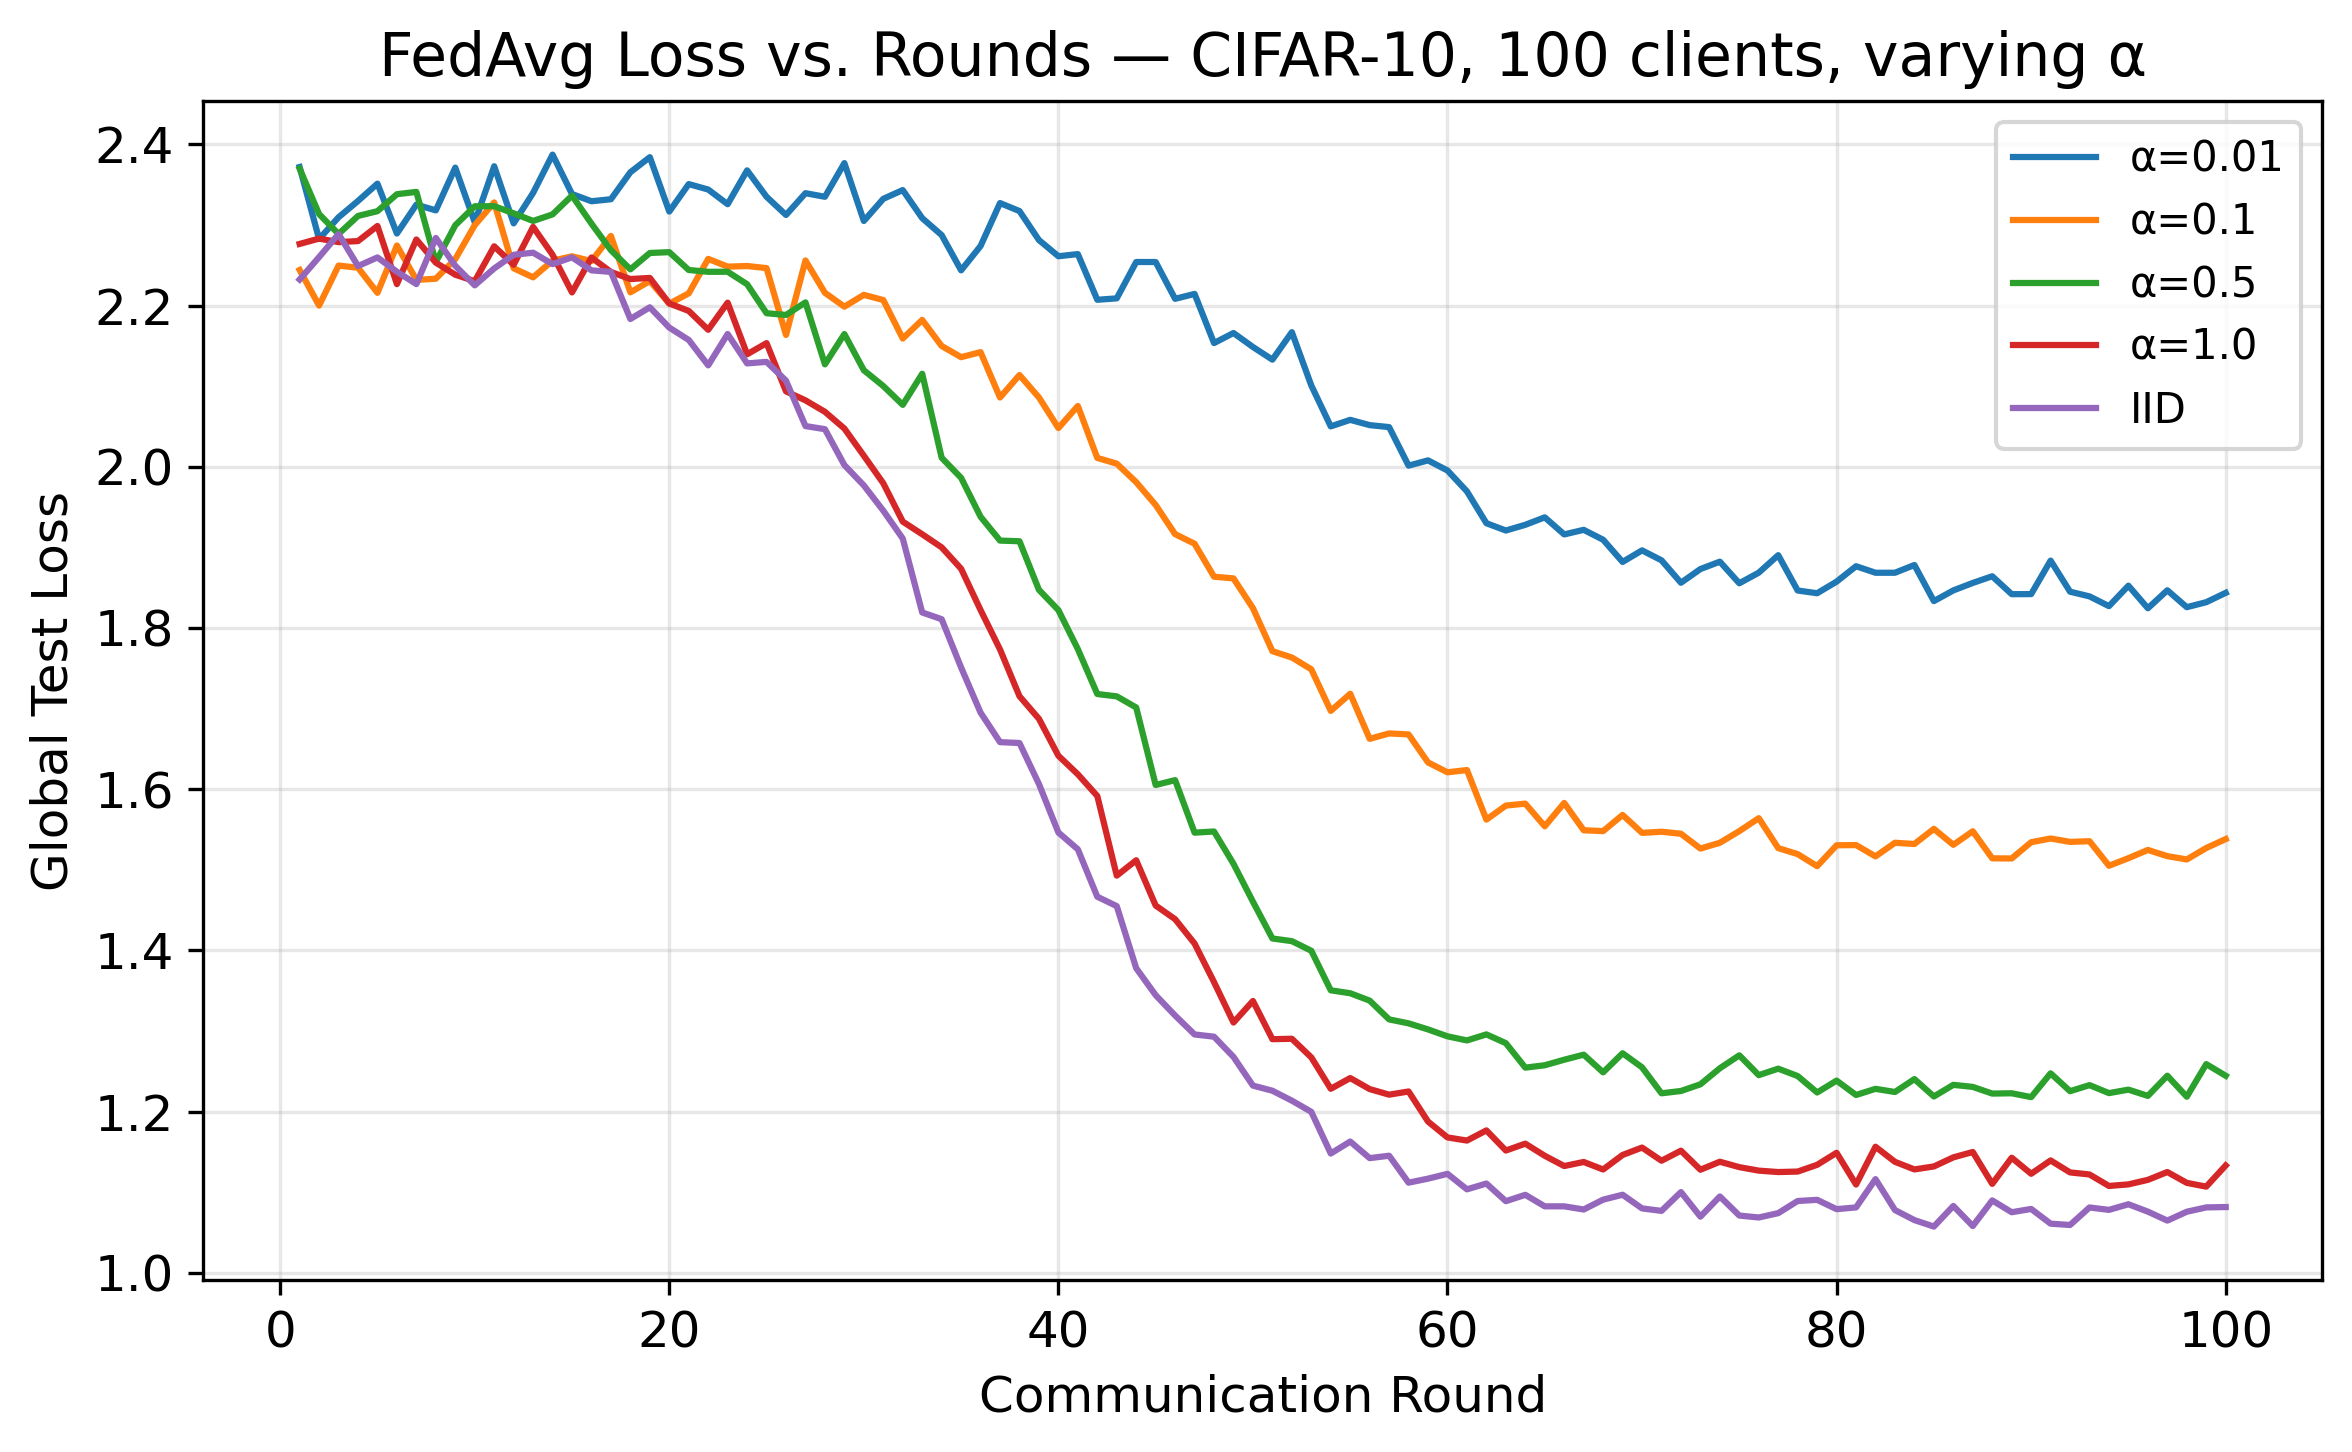
\includegraphics[width=\columnwidth]{loss_vs_alpha_cifar10_c100.png}
\caption{FedAvg loss vs.\ communication rounds on CIFAR-10 (100 clients). Higher heterogeneity ($\alpha=0.01$) leads to higher loss and noisier convergence.}
\label{fig:loss_alpha}
\end{figure}

\subsection{IID vs. Non-IID Comparison}

Figure~\ref{fig:iid_noniid} directly compares IID and non-IID ($\alpha=0.1$) performance on CIFAR-10.

\begin{figure}[h]
\centering
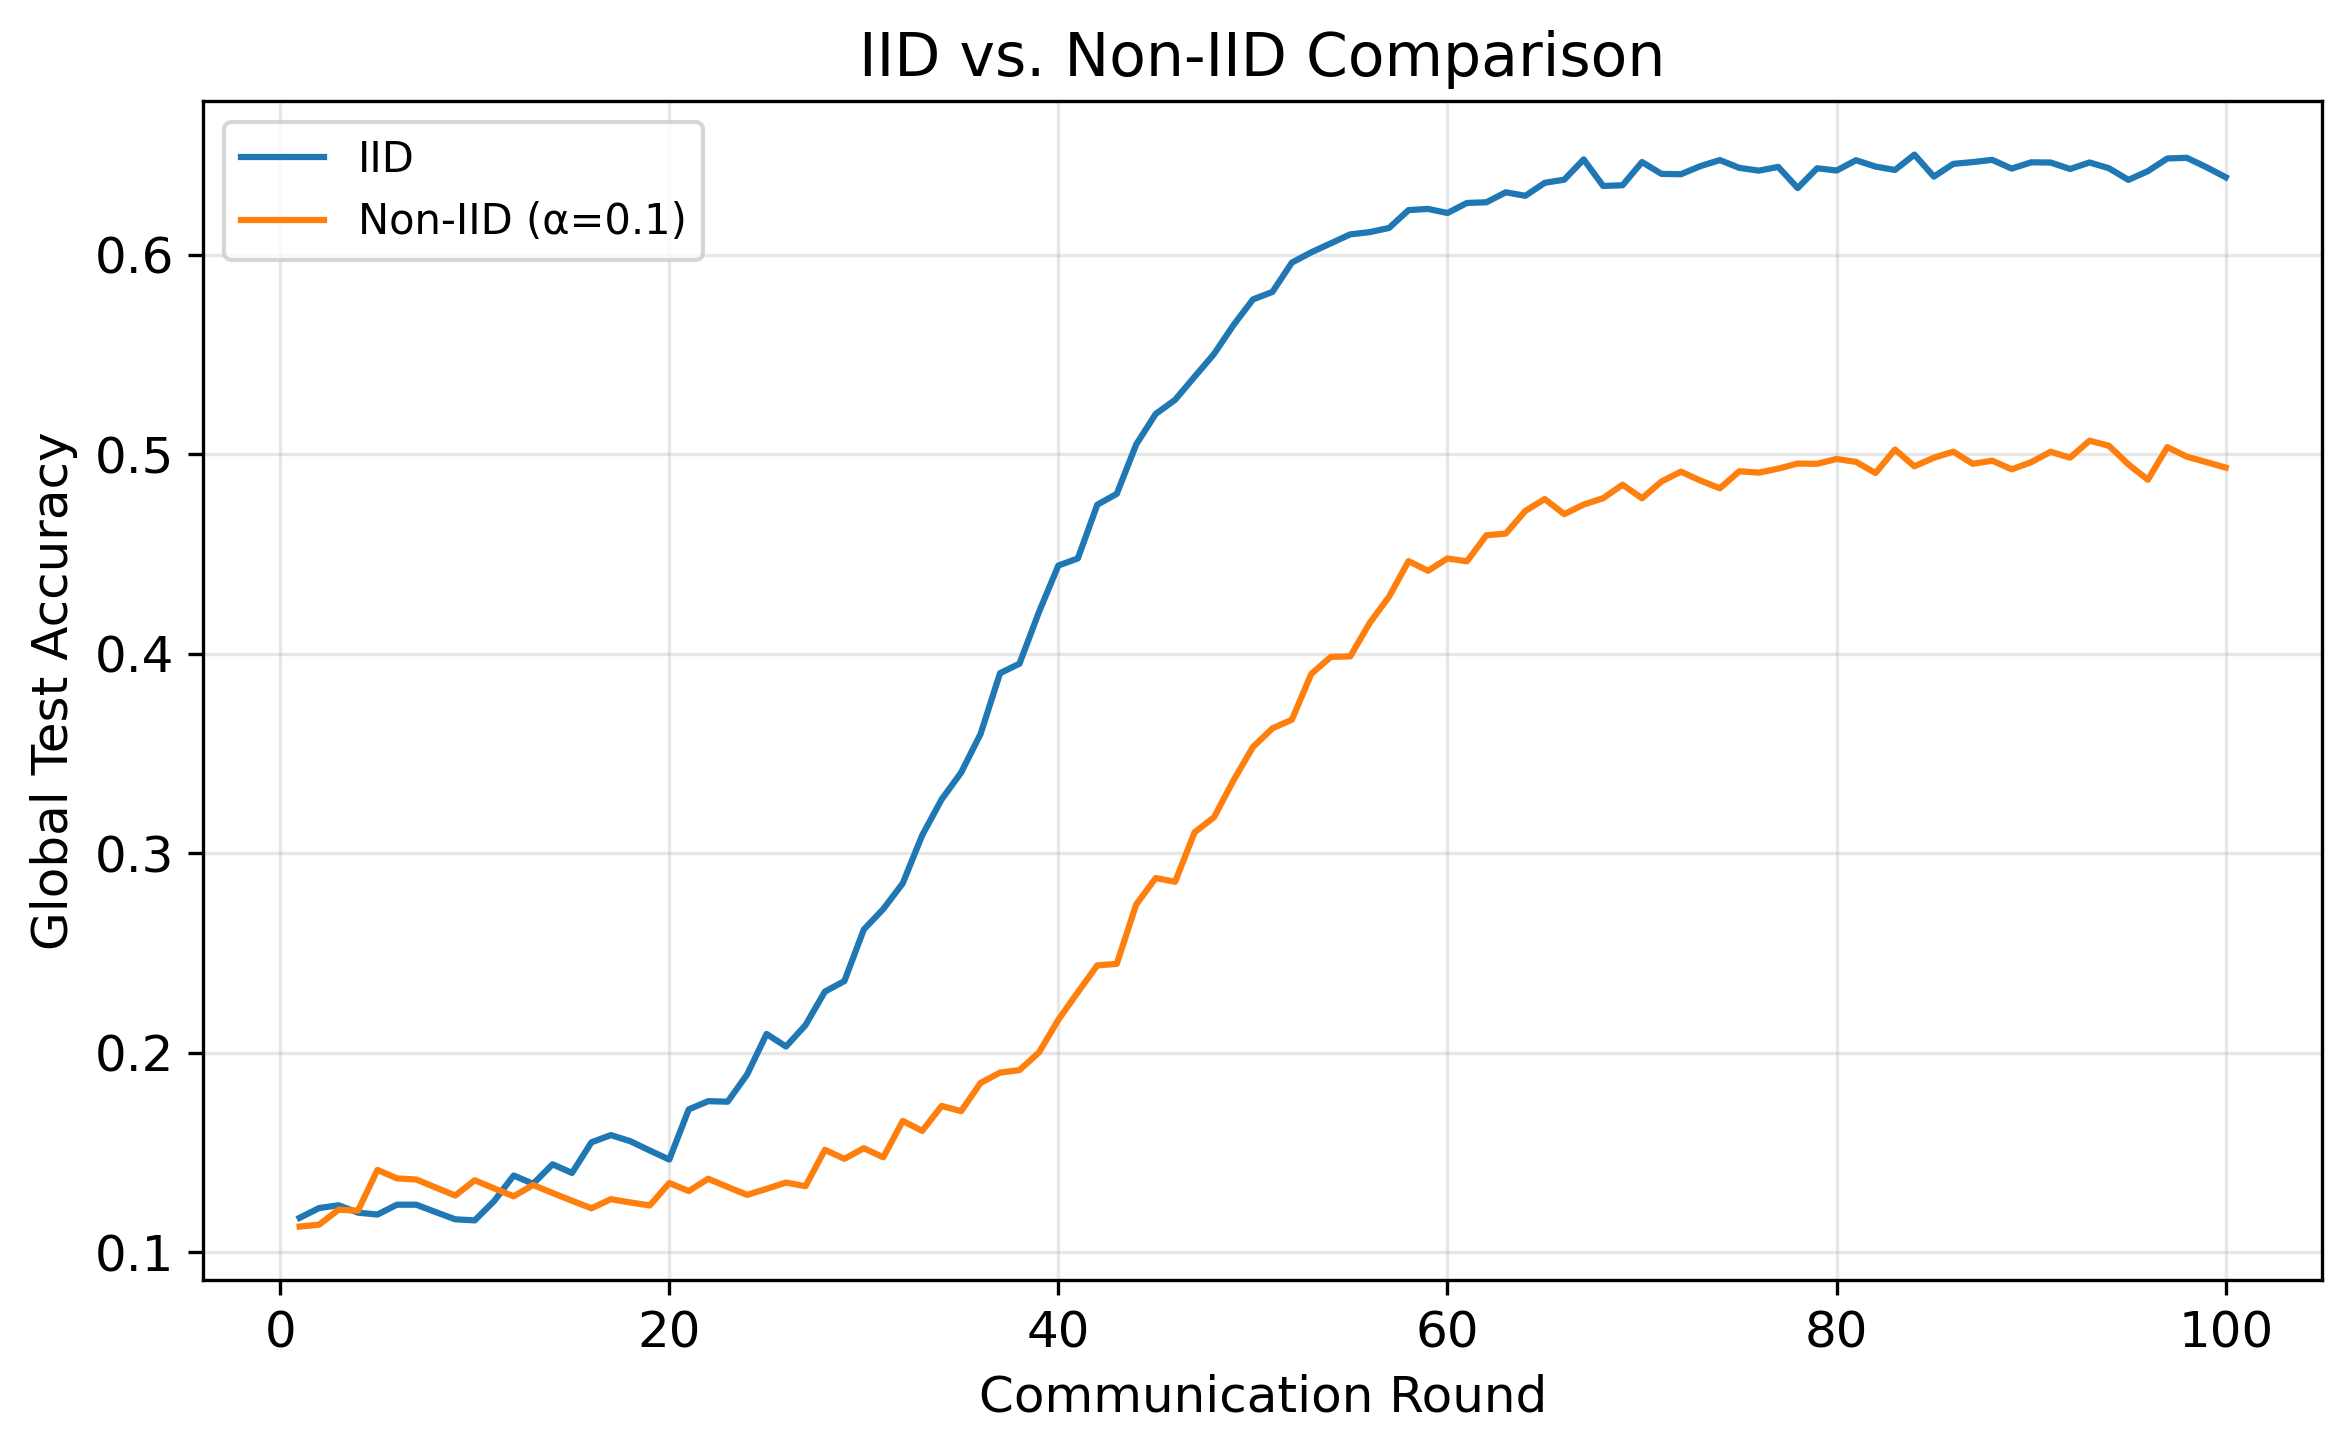
\includegraphics[width=\columnwidth]{iid_vs_noniid_cifar10.png}
\caption{IID vs.\ non-IID ($\alpha=0.1$) comparison on CIFAR-10 with 100 clients. The non-IID setting converges to substantially lower accuracy.}
\label{fig:iid_noniid}
\end{figure}

The gap between IID and non-IID performance is consistent across all datasets but varies in magnitude. MNIST, with its well-separated digit classes, shows a modest 3.17\% gap even at $\alpha=0.1$. Fashion-MNIST shows a 9.00\% gap, and CIFAR-10 shows a 14.55\% gap at the same $\alpha$. This suggests that \textbf{dataset complexity amplifies the effect of data heterogeneity}: when the task itself is harder, non-IID data distributions cause greater divergence between local models.

\subsection{Effect of Client Scale}

Figure~\ref{fig:clients} shows accuracy curves for different client counts on CIFAR-10 at $\alpha=0.1$.

\begin{figure}[h]
\centering
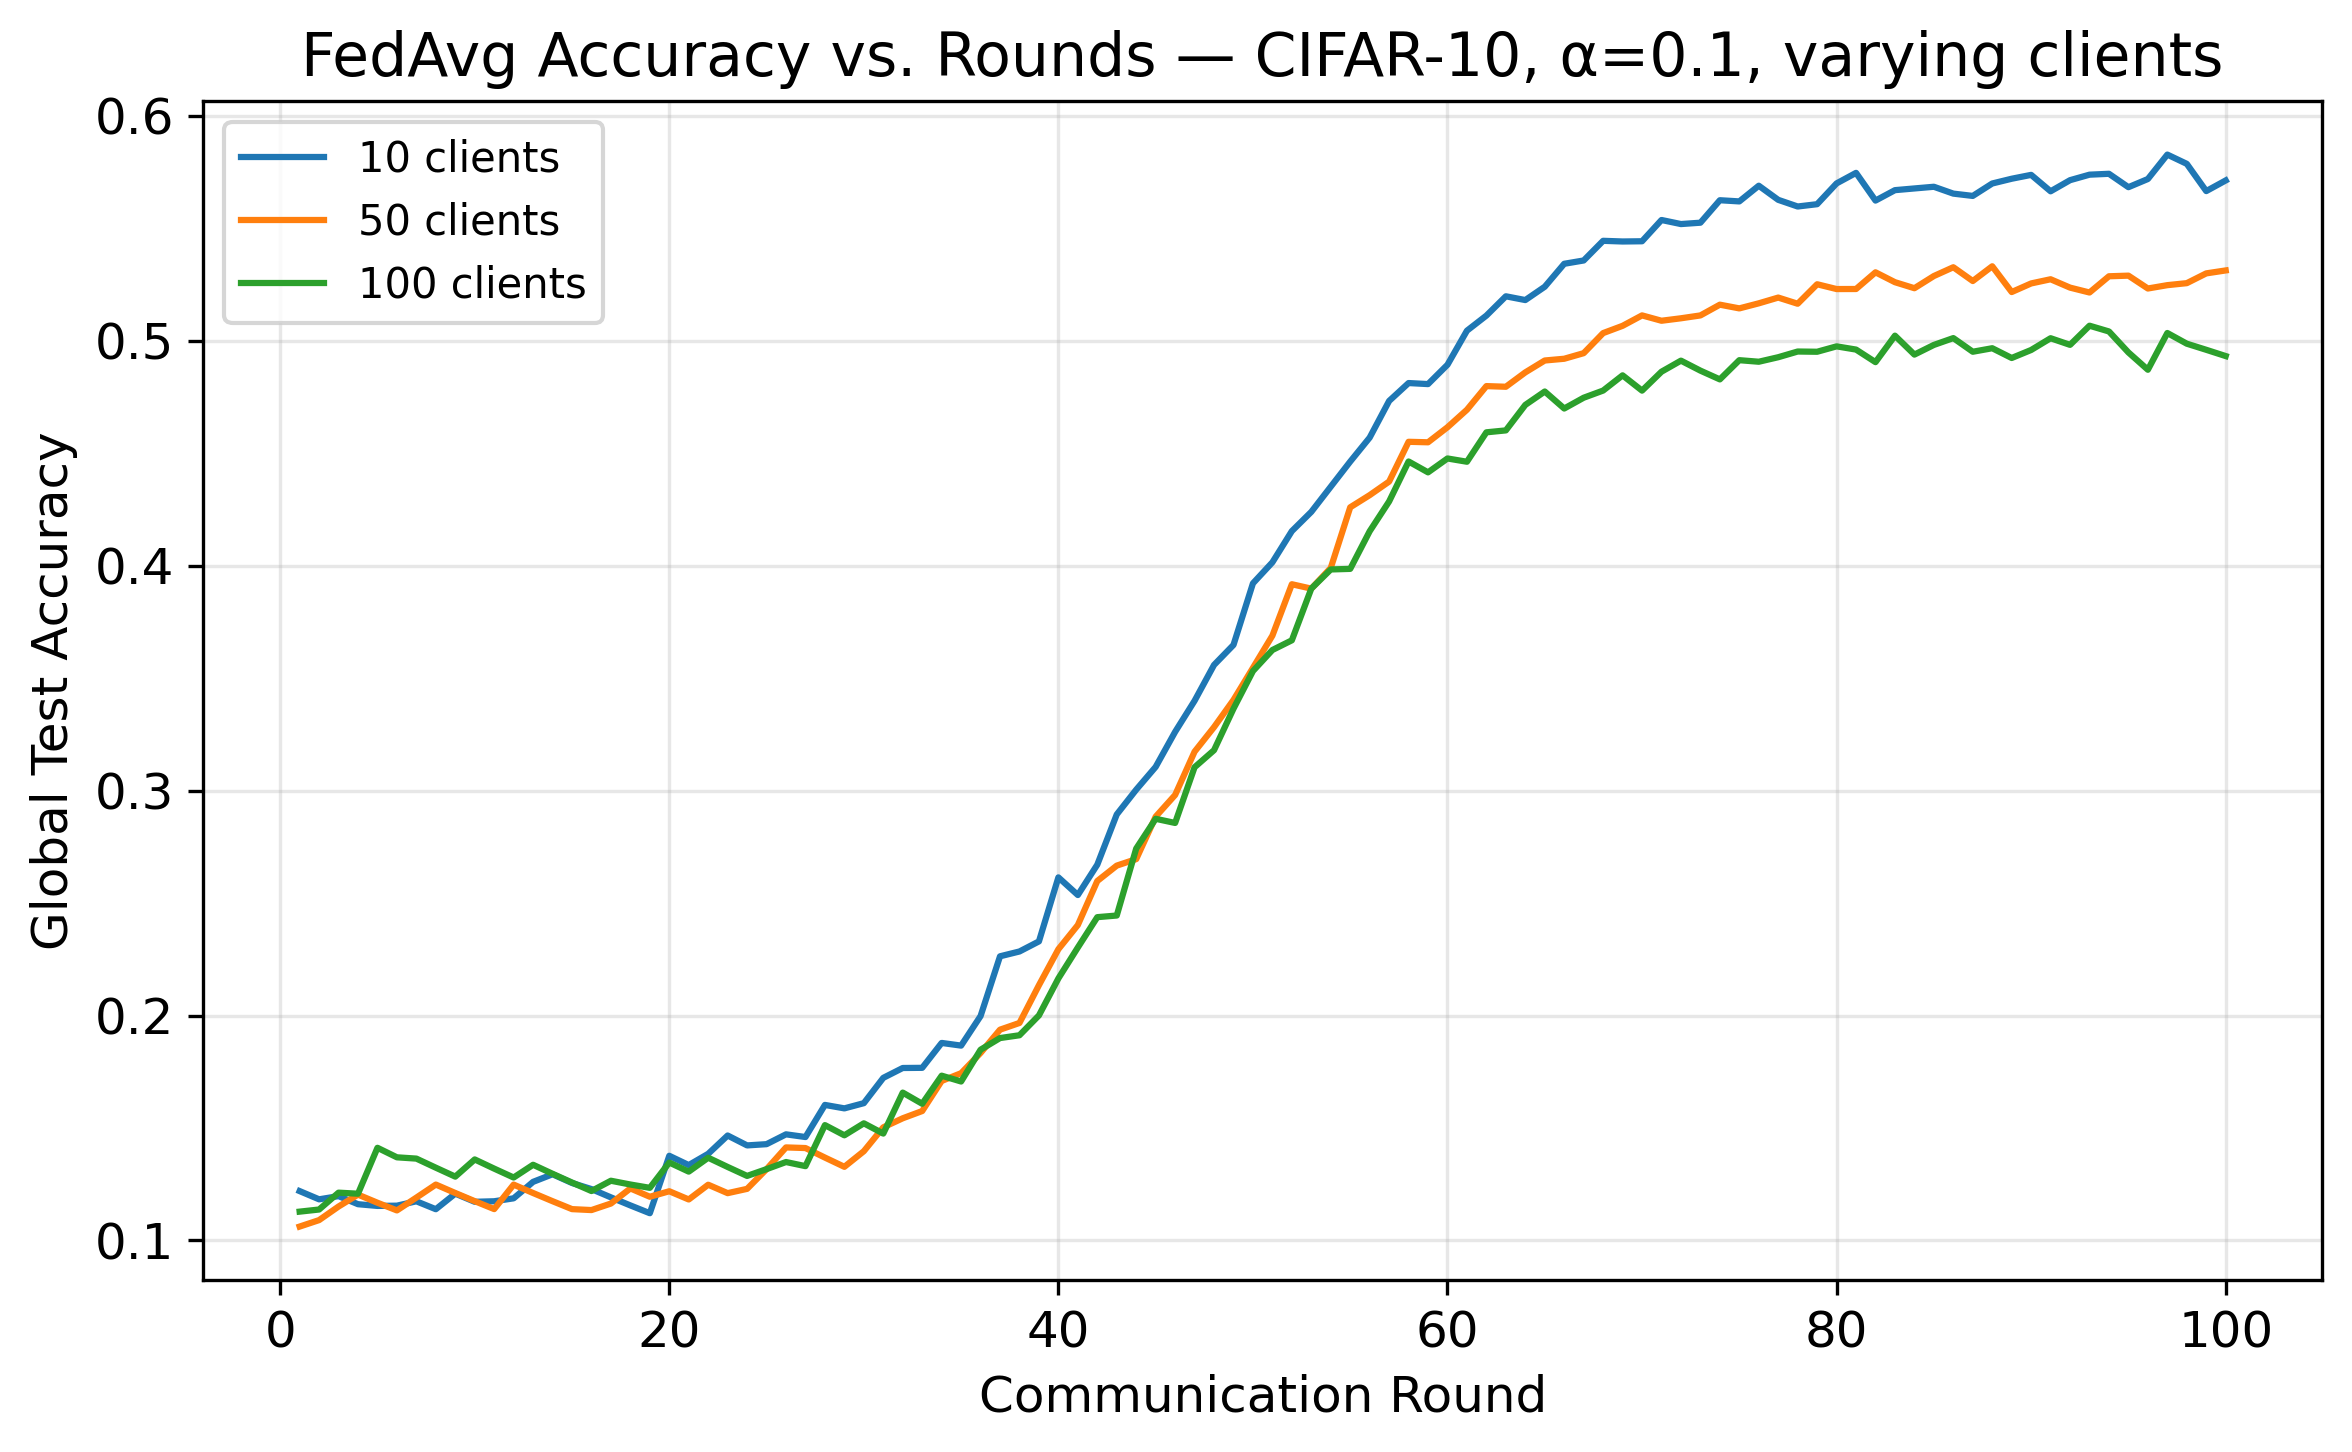
\includegraphics[width=\columnwidth]{accuracy_vs_clients_cifar10_a0.1.png}
\caption{FedAvg accuracy on CIFAR-10 ($\alpha=0.1$) with varying client counts. More clients with partial participation (50\%) degrades performance.}
\label{fig:clients}
\end{figure}

At $\alpha=0.1$ on CIFAR-10, accuracy drops from 57.13\% (10 clients) to 53.13\% (50 clients) to 49.32\% (100 clients). This degradation occurs because with more clients and a fixed participation fraction ($C=0.5$), each client holds less data (smaller local datasets) with higher label skew, and the subset of clients sampled each round becomes less representative of the global distribution. With 10 clients and 50\% participation, 5 clients contribute each round; with 100 clients, 50 contribute, but each holds only $\frac{1}{100}$th of the total data and has a more skewed label distribution.

Interestingly, under IID conditions, the effect is reversed for 10 vs.\ 50 clients (70.02\% vs.\ 66.14\%), suggesting that while more clients improve data diversity in principle, the reduced data per client and partial participation can still hurt convergence speed within a fixed round budget.

\subsection{Cross-Dataset Comparison}

Figure~\ref{fig:comparison} provides a bar chart comparing final test accuracies across datasets and heterogeneity levels.

\begin{figure}[h]
\centering
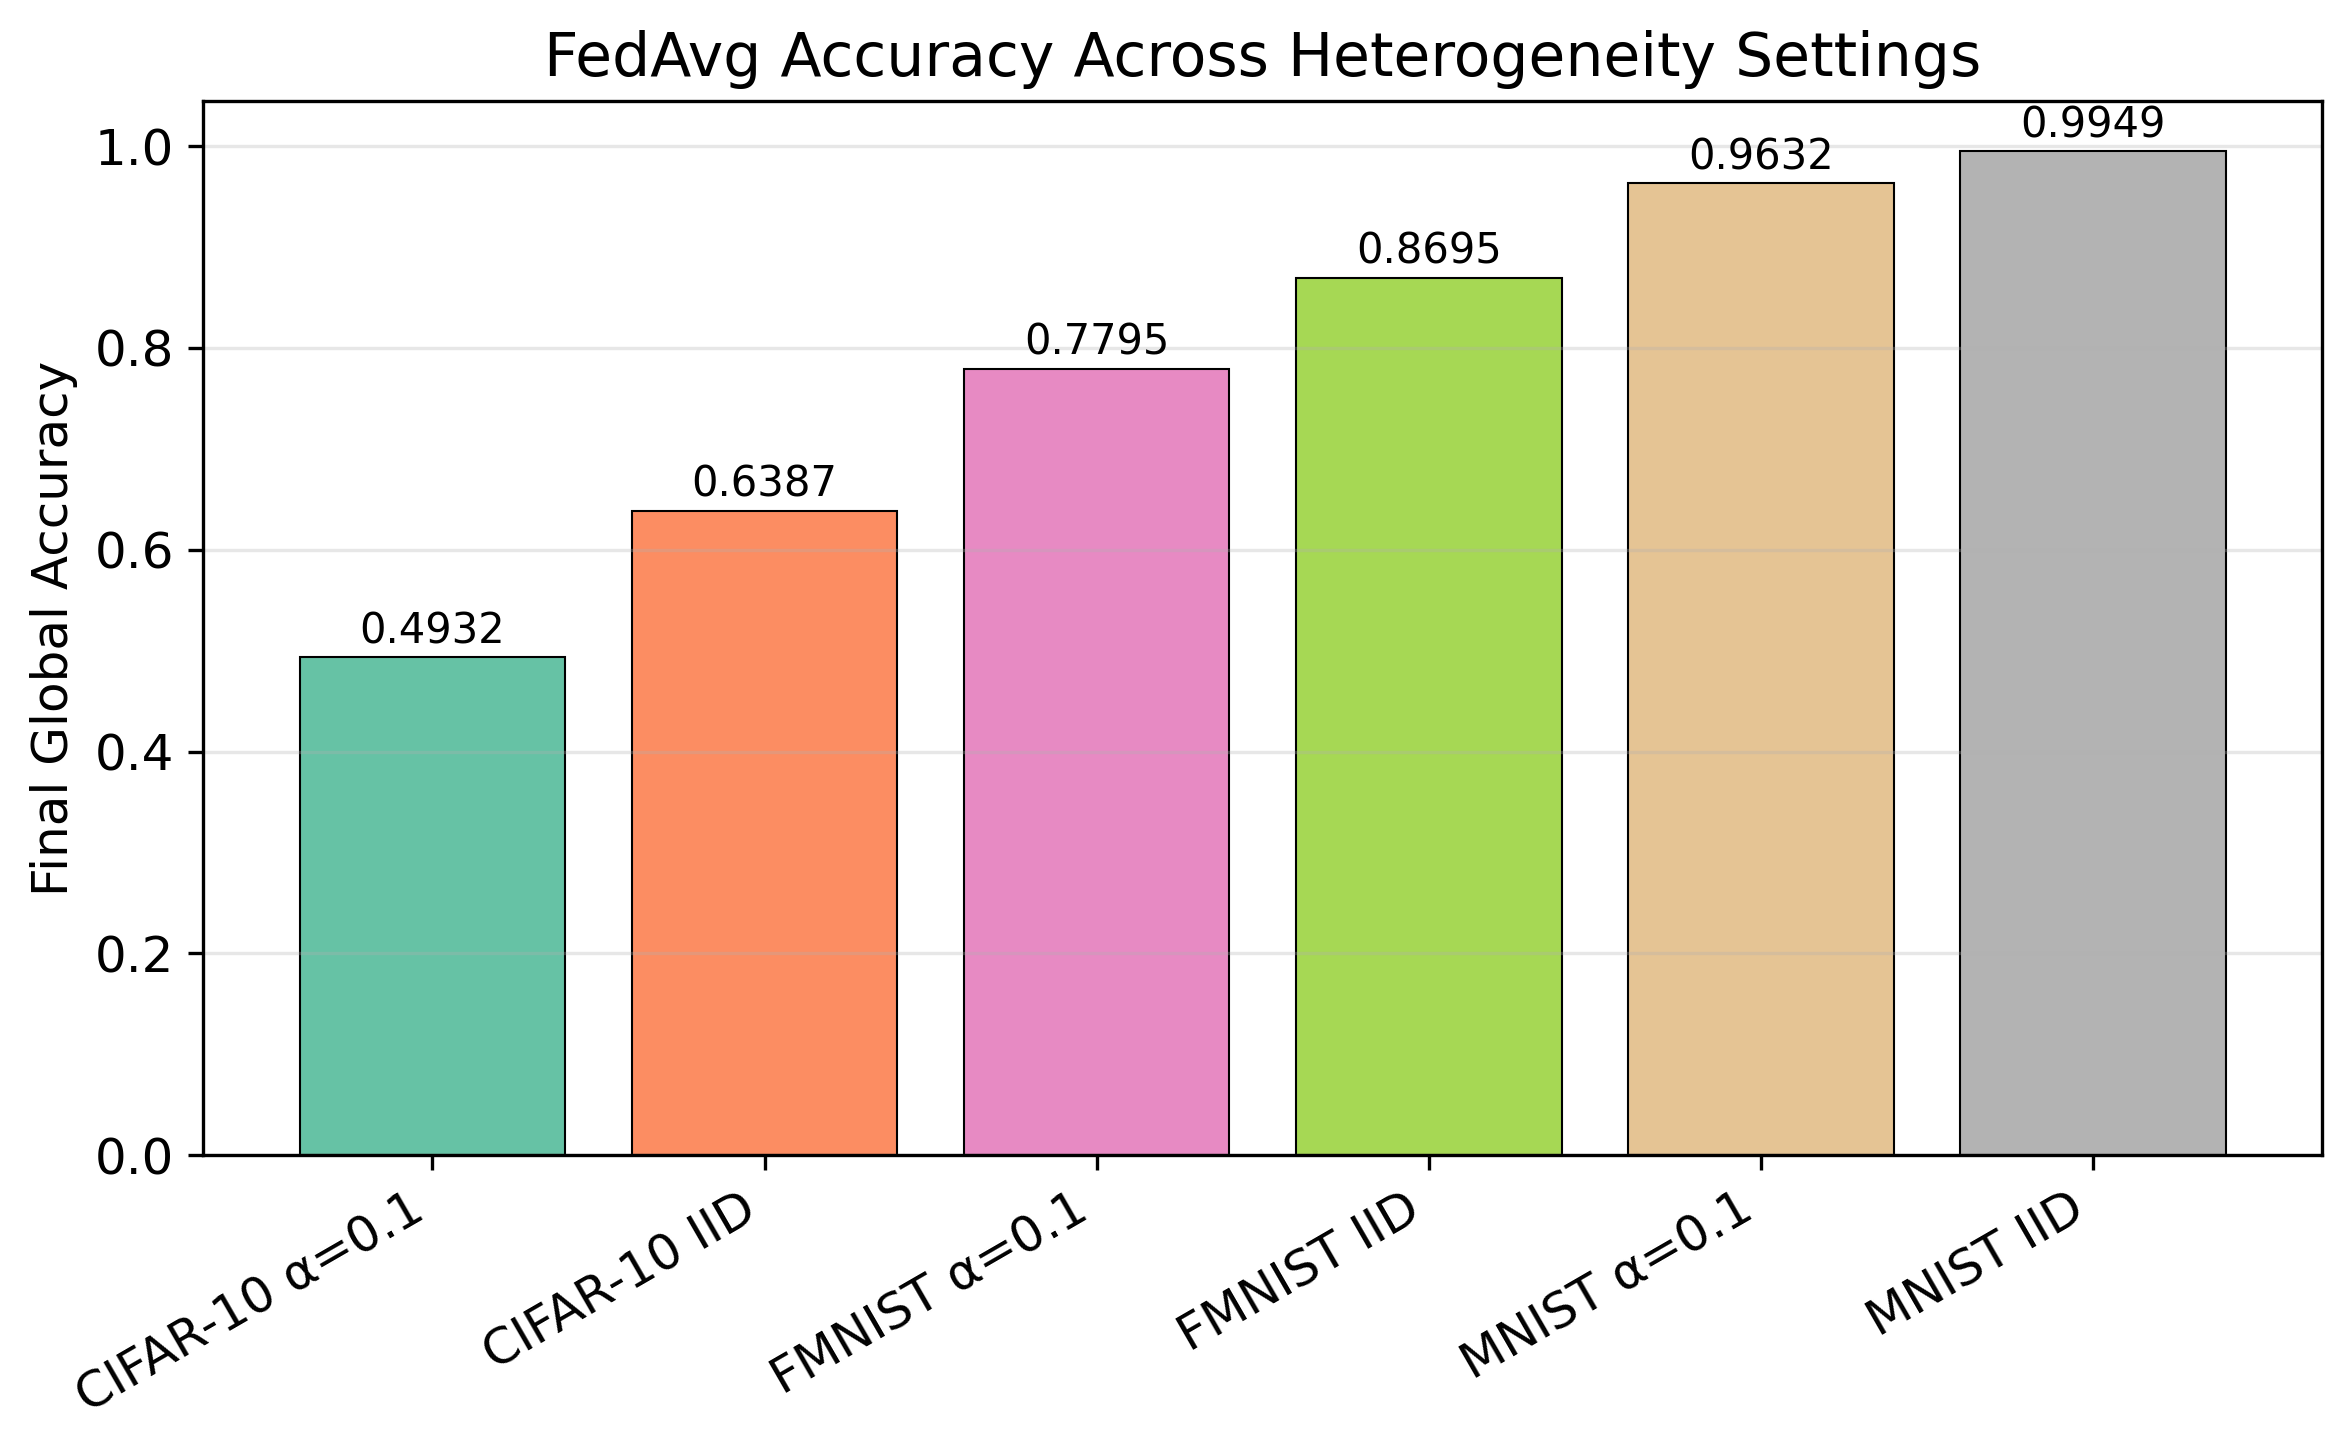
\includegraphics[width=\columnwidth]{accuracy_comparison.png}
\caption{Final test accuracy comparison across datasets and heterogeneity settings (100 clients). MNIST is robust to non-IID; CIFAR-10 is most affected.}
\label{fig:comparison}
\end{figure}

The cross-dataset comparison reveals a clear hierarchy: MNIST $>$ Fashion-MNIST $>$ CIFAR-10 in terms of both absolute accuracy and robustness to non-IID partitioning. This aligns with the intrinsic difficulty of each dataset and suggests that for complex tasks, additional techniques beyond FedAvg (proximal regularization, variance reduction, or personalization) are essential under heterogeneous conditions.

\subsection{Convergence Analysis}

Using an 80\% accuracy threshold, we observe that:
\begin{itemize}
    \item CIFAR-10 never reaches 80\% under any configuration within 100 rounds, indicating that this dataset-model combination needs either more rounds or algorithmic improvements.
    \item Fashion-MNIST converges at round 33--42 under IID/mild non-IID conditions but requires 87 rounds at $\alpha=0.1$ (50 clients) and fails to converge at $\alpha=0.1$ (100 clients).
    \item MNIST converges rapidly (round 16 for IID, round 24 for $\alpha=0.1$), confirming its limited diagnostic value for heterogeneity research.
\end{itemize}

The Fashion-MNIST results are particularly informative: they show a clear transition from ``easily convergent'' (IID, $\leq$35 rounds) to ``barely convergent'' ($\alpha=0.1$ at 50 clients, 87 rounds) to ``non-convergent'' ($\alpha=0.1$ at 100 clients) as heterogeneity and scale increase.


%% ============================================================
\section{Discussion}
\label{sec:discussion}

Our experimental findings quantify the well-known degradation of FedAvg under non-IID conditions and extend the analysis across the interaction of heterogeneity degree, client scale, and dataset complexity. Several key insights emerge:

\textbf{Non-linearity of heterogeneity impact.} The accuracy drop is not linear in $\alpha$. On CIFAR-10 (100 clients), the drop from IID to $\alpha=1.0$ is only 1.52\%, but from $\alpha=0.5$ to $\alpha=0.1$ it is 9.79\%, and from $\alpha=0.1$ to $\alpha=0.01$ it is 11.19\%. This suggests a critical threshold around $\alpha \approx 0.5$ below which heterogeneity effects accelerate.

\textbf{Client scale amplifies heterogeneity.} Increasing from 10 to 100 clients at $\alpha=0.1$ on CIFAR-10 causes an additional 7.81\% accuracy drop beyond the heterogeneity effect alone. This interaction between scale and non-IID is particularly concerning for real-world cross-device FL.

\textbf{Dataset complexity matters.} The same $\alpha$ value produces very different effects across datasets. At $\alpha=0.1$, the IID-to-non-IID gap is 3.17\% for MNIST, 9.00\% for FMNIST, and 14.55\% for CIFAR-10. This underscores the importance of evaluating FL methods on challenging datasets.

These findings contextualize the heterogeneity taxonomy of Chen et al.~\cite{chen2025advances} with concrete empirical evidence and motivate the development of methods that specifically target the identified failure modes.


%% ============================================================
\section{Conclusion}
\label{sec:conclusion}

We conducted a systematic experimental evaluation of FedAvg under varying data heterogeneity conditions, guided by the heterogeneity taxonomy of Chen et al.~\cite{chen2025advances}. Our 22 experiments across MNIST, Fashion-MNIST, and CIFAR-10 with 10--100 clients and Dirichlet $\alpha$ values from 0.01 to IID reveal that:

\begin{enumerate}
    \item Data heterogeneity causes significant accuracy degradation, up to 25.74\% on CIFAR-10 at extreme non-IID ($\alpha=0.01$).
    \item The degradation is non-linear, with a critical threshold around $\alpha \approx 0.5$ below which performance drops accelerate.
    \item Larger client populations amplify the non-IID effect due to smaller per-client datasets and partial participation.
    \item Dataset complexity multiplicatively interacts with heterogeneity---complex tasks suffer disproportionately.
\end{enumerate}

These results establish clear baselines for where FedAvg succeeds (simple tasks, mild heterogeneity) and where it fails (complex tasks, $\alpha < 0.5$, large client populations). The identified failure modes directly motivate the techniques surveyed in~\cite{chen2025advances}: proximal regularization (FedProx~\cite{li2020federated}), variance reduction (SCAFFOLD~\cite{karimireddy2020scaffold}), client selection~\cite{lai2021oort}, and asynchronous aggregation~\cite{nguyen2022federated,wang2025decentralized} as necessary tools for practical heterogeneous FL deployments.

Future work could extend this analysis to feature and quantity skew (beyond label skew), evaluate the surveyed methods under identical conditions for direct comparison, and investigate the interaction of data heterogeneity with system heterogeneity (stragglers) and communication constraints.


%% ============================================================
\bibliographystyle{IEEEtran}
\bibliography{references}

\end{document}
